Для передачи информации радиоволну необходимо модулировать сигналом, содержащим информацию. Длинные, средние и короткие волны обычно имеют амплитудную модуляцию <<AM>>. Ультракороткие волны обычно имеют частотную модуляцию <<FM>>.

Модуляция (лат. modulatio --- размеренность, ритмичность) --- процесс изменения одного или нескольких параметров высокочастотного несущего колебания по закону низкочастотного информационного сигнала (сообщения)~\cite{wiki:modulation}.

Передаваемая информация заложена в управляющем (модулирующем) сигнале, а роль переносчика информации выполняет высокочастотное колебание, называемое несущим. Модуляция, таким образом, представляет собой процесс <<посадки>> информационного колебания на заведомо известную несущую.

В результате модуляции спектр низкочастотного управляющего сигнала переносится в область высоких частот. Это позволяет при организации вещания настроить функционирование всех приёмо-передающих устройств на разных частотах с тем, чтобы они <<не мешали>> друг другу.

Амплитудная модуляция представлена на рисунке~\ref{fig:am}. Этот тип модуляции изменяет \textbf{амплитуду} несущей частоты под действием кодирующего колебания (сигнала). Главный её недостаток --- низкая помехоустойчивость.

\begin{figure}[ht]
    \subfloat[]{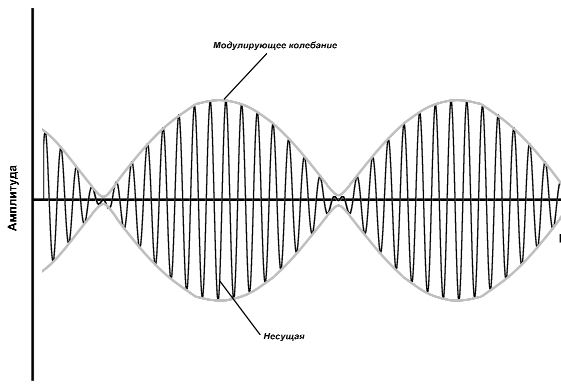
\includegraphics[width=.6\linewidth]{Figures/am.jpg}}
    \subfloat[]{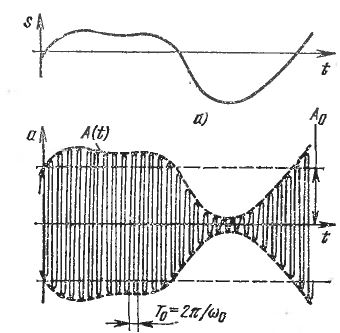
\includegraphics[width=.4\linewidth]{Figures/amclose.jpg}}
    \caption{Амплитудная модуляция (а) общая картина; (б) изменение несущего колебания по заданному закону}
    \label{fig:am}
\end{figure}

Частотная модуляция (рисунок~\ref{fig:fm}) --- изменение несущей \textbf{частоты} под воздействием кодирующего сигнала. Этот вид модуляции имеет более высокую помехоустойчивость несмотря на свою аналоговую природу.

\begin{figure}[ht]
    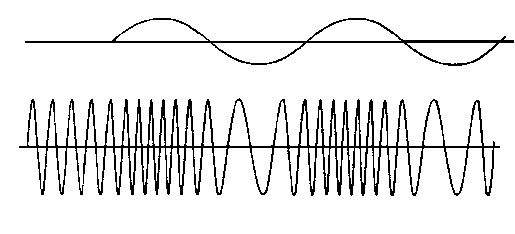
\includegraphics[width=.8\linewidth]{Figures/fm.jpg}
    \caption{Частотная модуляция}
    \label{fig:fm}
\end{figure}

Фазовая модуляция (рисунок~\ref{fig:pm}) --- изменение фазы несущей частоты скачкообразно (манипуляция). Недостаток данной модуляции в том, что ошибка в одном символе может привести к некорректному приёму всех последующих.

\begin{figure}[ht]
    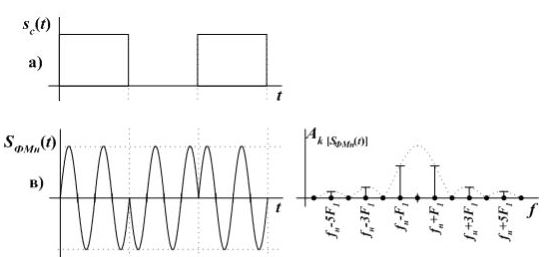
\includegraphics[width=.8\linewidth]{Figures/pm.jpg}
    \caption{Фазовая модуляция}
    \label{fig:pm}
\end{figure}

Дифференциально-фазовая манипуляция --- изменение фазы несущей частоты только при изменении разности (в данном случае --- при приходе каждой <<1>>).
